\section{Příklad 4}
% Jako parametr zadejte skupinu (A-H)
\ctvrtyZadani{E}
\newline
\Large{Do obvodu si znázorníme smyčkové proudy:}
\begin{center}
    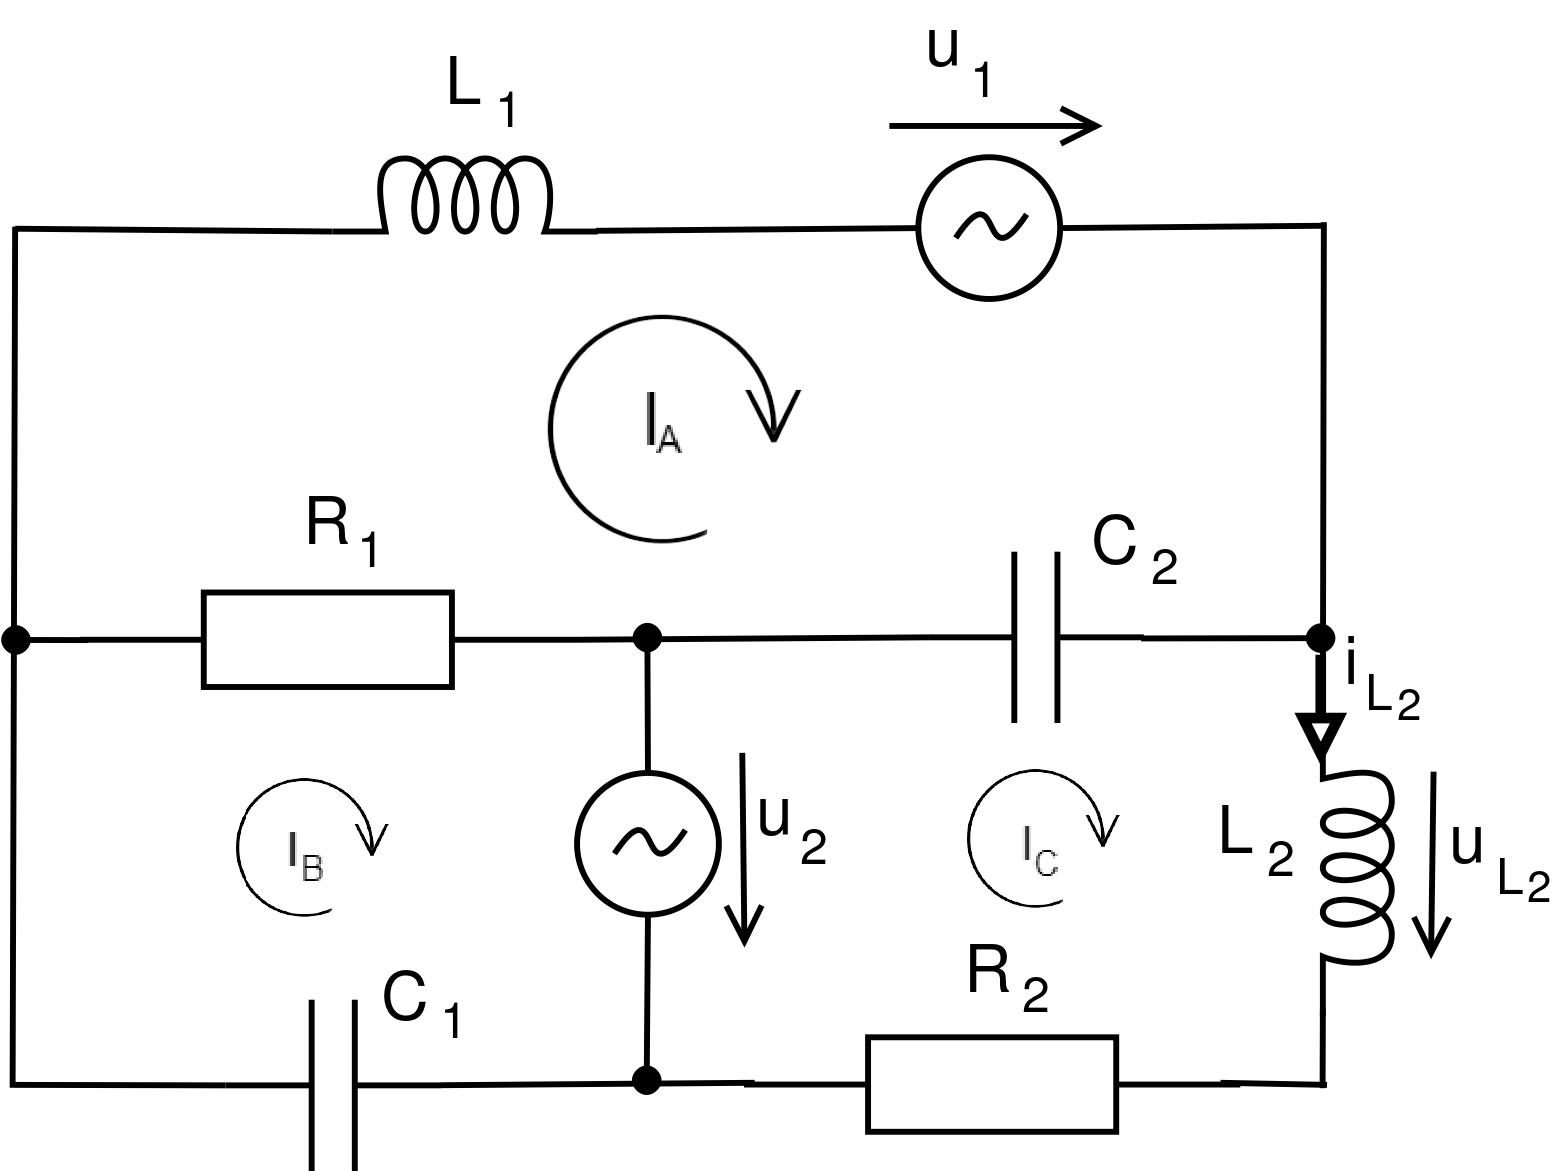
\includegraphics[scale=0.6,keepaspectratio]{fig/Pr4Arrows.jpg}
\end{center}
\newpage
\noindent{\Large{Vyjádříme si úhlovou rychlost $\omega$}:}\\
\begin{math}
\newline
    \omega = 2\pi f = 2\pi \cdot 90 = 180\pi\:rad/s\\\\
\end{math}
\Large{Sestavíme rovnice pro jednotlivé smyčky:}\\
\begin{math}
\newline
    I_A)\quad L_1\omega i I_A + U_1 + \frac{1}{C_1\omega i}(I_A-I_C) + R_1(I_A-I_B) = 0\\
    I_B)\quad R_1(I_B-I_A)+U_2+\frac{1}{C_1\omega i}I_B = 0\\
    I_C)\quad \frac{1}{\omega C_2 i}(I_C-I_A)+L_2\omega iI_C+R_2I_C-U2=0\\ \\
\end{math}
\Large{Upravíme a sestavíme matici:}\\
\begin{math}
\newline
\begin{pmatrix}
R_1-\frac{1}{\omega C_2}i+\omega L_1i & -R_1 & \frac{1}{\omega C_2}i\\
-R_1 & R_1 - \frac{1}{\omega C_1}i & 0\\
\frac{1}{\omega C_2}i & 0 & R_2-\frac{1}{\omega C_2}i+\omega L_2i
\end{pmatrix}
\begin{pmatrix}
I_A\\
I_B\\
I_C
\end{pmatrix}
=
\begin{pmatrix}
-U_1\\
-U_2\\
U_2
\end{pmatrix}\\ \\
%matice s dosazenim
\newline
\begin{pmatrix}
14+46,3073i & -14 & 27,2060i\\
-14 & 14-17,6839i & 0\\
27,2060i & 0 & 13+6,7232i
\end{pmatrix}
\begin{pmatrix}
I_A\\
I_B\\
I_C
\end{pmatrix}
=
\begin{pmatrix}
-5\\
-3\\
3
\end{pmatrix}\\ \\
\newline
\end{math}
\Large{Uplatníme Cramerovo a Sarusovo pravidlo pro výpočet determinantů a získáme hoddnotu \(I_C\):}\\ 
\begin{math}
\newline
\Delta \doteq  18313,7316 - 2373,9271i\\
\Delta_C \doteq 4862,2145 + 4249,2523i\\ \\
I_C = \frac{\Delta_C}{\Delta}\quad \quad I_C \doteq \frac{4862,2145 + 4249,2523i}{18313,7316 - 2373,9271i} \doteq 0,2315+0,2620i\:A\\ \\
\end{math}
\huge{\[I_{L2} \equiv I_C\]} \\
\Large{Vypočítáme napětí na cívce \(U_{L2}\):}\\ 
\begin{math}
\newline
    Z_{L2} = \omega L_2i\quad\quad Z_{L2} = 180\pi\cdot 60 \cdot 10^{-3}i=\frac{54\pi}{5}i\:\Omega\\ \\
    U_{L2} = I_{L2}Z_{L2}\quad\quad U_{L2}= (0,2315+0,2620i)\cdot\frac{54}{5}i=-8,8907+7,8556i\:V\\ \\
\end{math}
\Large{Dopočítáme \(|U_{L_2}|\) a \(\varphi_{L_2}\):}\\
\begin{math}
\newline
    |U_{L_2}|= \sqrt{Re(U_{L_2})^2+Im(U_{L_2})^2}\quad\quad|U_{L_2}|=\sqrt{(-8,8907)^2+7,8556^2}\doteq\underline{11,8640}\:V\\\\
    \varphi_{L_2}=\arctan{\frac{Im(U_{L_2})}{Re(U_{L_2})}}\quad\quad\varphi_{L_2}=\arctan{\frac{7,8556}{-8,8907}}\doteq\underline{-0,7237}\:rad\\
\end{math}